\documentclass[1p]{elsarticle_modified}
%\bibliographystyle{elsarticle-num}

%\usepackage[colorlinks]{hyperref}
%\usepackage{abbrmath_seonhwa} %\Abb, \Ascr, \Acal ,\Abf, \Afrak
\usepackage{amsfonts}
\usepackage{amssymb}
\usepackage{amsmath}
\usepackage{amsthm}
\usepackage{scalefnt}
\usepackage{amsbsy}
\usepackage{kotex}
\usepackage{caption}
\usepackage{subfig}
\usepackage{color}
\usepackage{graphicx}
\usepackage{xcolor} %% white, black, red, green, blue, cyan, magenta, yellow
\usepackage{float}
\usepackage{setspace}
\usepackage{hyperref}

\usepackage{tikz}
\usetikzlibrary{arrows}

\usepackage{multirow}
\usepackage{array} % fixed length table
\usepackage{hhline}

%%%%%%%%%%%%%%%%%%%%%
\makeatletter
\renewcommand*\env@matrix[1][\arraystretch]{%
	\edef\arraystretch{#1}%
	\hskip -\arraycolsep
	\let\@ifnextchar\new@ifnextchar
	\array{*\c@MaxMatrixCols c}}
\makeatother %https://tex.stackexchange.com/questions/14071/how-can-i-increase-the-line-spacing-in-a-matrix
%%%%%%%%%%%%%%%

\usepackage[normalem]{ulem}

\newcommand{\msout}[1]{\ifmmode\text{\sout{\ensuremath{#1}}}\else\sout{#1}\fi}
%SOURCE: \msout is \stkout macro in https://tex.stackexchange.com/questions/20609/strikeout-in-math-mode

\newcommand{\cancel}[1]{
	\ifmmode
	{\color{red}\msout{#1}}
	\else
	{\color{red}\sout{#1}}
	\fi
}

\newcommand{\add}[1]{
	{\color{blue}\uwave{#1}}
}

\newcommand{\replace}[2]{
	\ifmmode
	{\color{red}\msout{#1}}{\color{blue}\uwave{#2}}
	\else
	{\color{red}\sout{#1}}{\color{blue}\uwave{#2}}
	\fi
}

\newcommand{\Sol}{\mathcal{S}} %segment
\newcommand{\D}{D} %diagram
\newcommand{\A}{\mathcal{A}} %arc


%%%%%%%%%%%%%%%%%%%%%%%%%%%%%5 test

\def\sl{\operatorname{\textup{SL}}(2,\Cbb)}
\def\psl{\operatorname{\textup{PSL}}(2,\Cbb)}
\def\quan{\mkern 1mu \triangleright \mkern 1mu}

\theoremstyle{definition}
\newtheorem{thm}{Theorem}[section]
\newtheorem{prop}[thm]{Proposition}
\newtheorem{lem}[thm]{Lemma}
\newtheorem{ques}[thm]{Question}
\newtheorem{cor}[thm]{Corollary}
\newtheorem{defn}[thm]{Definition}
\newtheorem{exam}[thm]{Example}
\newtheorem{rmk}[thm]{Remark}
\newtheorem{alg}[thm]{Algorithm}

\newcommand{\I}{\sqrt{-1}}
\begin{document}

%\begin{frontmatter}
%
%\title{Boundary parabolic representations of knots up to 8 crossings}
%
%%% Group authors per affiliation:
%\author{Yunhi Cho} 
%\address{Department of Mathematics, University of Seoul, Seoul, Korea}
%\ead{yhcho@uos.ac.kr}
%
%
%\author{Seonhwa Kim} %\fnref{s_kim}}
%\address{Center for Geometry and Physics, Institute for Basic Science, Pohang, 37673, Korea}
%\ead{ryeona17@ibs.re.kr}
%
%\author{Hyuk Kim}
%\address{Department of Mathematical Sciences, Seoul National University, Seoul 08826, Korea}
%\ead{hyukkim@snu.ac.kr}
%
%\author{Seokbeom Yoon}
%\address{Department of Mathematical Sciences, Seoul National University, Seoul, 08826,  Korea}
%\ead{sbyoon15@snu.ac.kr}
%
%\begin{abstract}
%We find all boundary parabolic representation of knots up to 8 crossings.
%
%\end{abstract}
%\begin{keyword}
%    \MSC[2010] 57M25 
%\end{keyword}
%
%\end{frontmatter}

%\linenumbers
%\tableofcontents
%
\newcommand\colored[1]{\textcolor{white}{\rule[-0.35ex]{0.8em}{1.4ex}}\kern-0.8em\color{red} #1}%
%\newcommand\colored[1]{\textcolor{white}{ #1}\kern-2.17ex	\textcolor{white}{ #1}\kern-1.81ex	\textcolor{white}{ #1}\kern-2.15ex\color{red}#1	}

{\Large $\underline{11n_{112}~(K11n_{112})}$}

\setlength{\tabcolsep}{10pt}
\renewcommand{\arraystretch}{1.6}
\vspace{1cm}\begin{tabular}{m{100pt}>{\centering\arraybackslash}m{274pt}}
\multirow{5}{120pt}{
	\centering
	\includegraphics[width=112pt]{../../../GIT/diagram.site/Diagrams/png/728_11n_112.png}\\
\ \ \ A knot diagram\footnotemark}&
\allowdisplaybreaks
\textbf{Linearized knot diagam} \\
\cline{2-2}
 &
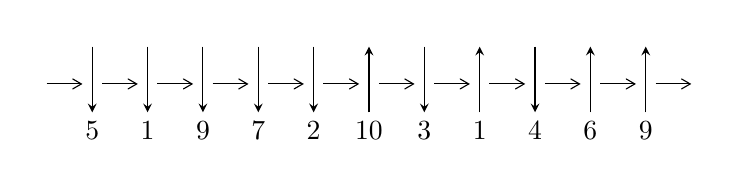
\begin{tikzpicture}[x=20pt, y=17pt]
	% nodes
	\node (C0) at (0, 0) {};
	\node (C1) at (1, 0) {};
	\node (C1U) at (1, +1) {};
	\node (C1D) at (1, -1) {5};

	\node (C2) at (2, 0) {};
	\node (C2U) at (2, +1) {};
	\node (C2D) at (2, -1) {1};

	\node (C3) at (3, 0) {};
	\node (C3U) at (3, +1) {};
	\node (C3D) at (3, -1) {9};

	\node (C4) at (4, 0) {};
	\node (C4U) at (4, +1) {};
	\node (C4D) at (4, -1) {7};

	\node (C5) at (5, 0) {};
	\node (C5U) at (5, +1) {};
	\node (C5D) at (5, -1) {2};

	\node (C6) at (6, 0) {};
	\node (C6U) at (6, +1) {};
	\node (C6D) at (6, -1) {10};

	\node (C7) at (7, 0) {};
	\node (C7U) at (7, +1) {};
	\node (C7D) at (7, -1) {3};

	\node (C8) at (8, 0) {};
	\node (C8U) at (8, +1) {};
	\node (C8D) at (8, -1) {1};

	\node (C9) at (9, 0) {};
	\node (C9U) at (9, +1) {};
	\node (C9D) at (9, -1) {4};

	\node (C10) at (10, 0) {};
	\node (C10U) at (10, +1) {};
	\node (C10D) at (10, -1) {6};

	\node (C11) at (11, 0) {};
	\node (C11U) at (11, +1) {};
	\node (C11D) at (11, -1) {9};
	\node (C12) at (12, 0) {};

	% arrows
	\draw[->,>={angle 60}]
	(C0) edge (C1) (C1) edge (C2) (C2) edge (C3) (C3) edge (C4) (C4) edge (C5) (C5) edge (C6) (C6) edge (C7) (C7) edge (C8) (C8) edge (C9) (C9) edge (C10) (C10) edge (C11) (C11) edge (C12) ;	\draw[->,>=stealth]
	(C1U) edge (C1D) (C2U) edge (C2D) (C3U) edge (C3D) (C4U) edge (C4D) (C5U) edge (C5D) (C6D) edge (C6U) (C7U) edge (C7D) (C8D) edge (C8U) (C9U) edge (C9D) (C10D) edge (C10U) (C11D) edge (C11U) ;
	\end{tikzpicture} \\
\hhline{~~} \\& 
\textbf{Solving Sequence} \\ \cline{2-2} 
 &
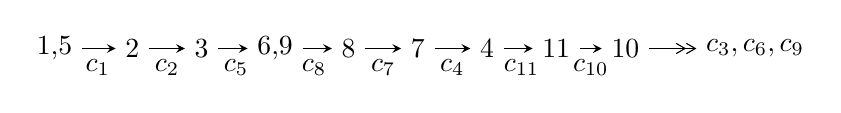
\begin{tikzpicture}[x=25pt, y=7pt]
	% node
	\node (A0) at (-1/8, 0) {1,5};
	\node (A1) at (1, 0) {2};
	\node (A2) at (2, 0) {3};
	\node (A3) at (49/16, 0) {6,9};
	\node (A4) at (33/8, 0) {8};
	\node (A5) at (41/8, 0) {7};
	\node (A6) at (49/8, 0) {4};
	\node (A7) at (57/8, 0) {11};
	\node (A8) at (65/8, 0) {10};
	\node (C1) at (1/2, -1) {$c_{1}$};
	\node (C2) at (3/2, -1) {$c_{2}$};
	\node (C3) at (5/2, -1) {$c_{5}$};
	\node (C4) at (29/8, -1) {$c_{8}$};
	\node (C5) at (37/8, -1) {$c_{7}$};
	\node (C6) at (45/8, -1) {$c_{4}$};
	\node (C7) at (53/8, -1) {$c_{11}$};
	\node (C8) at (61/8, -1) {$c_{10}$};
	\node (A9) at (10, 0) {$c_{3},c_{6},c_{9}$};

	% edge
	\draw[->,>=stealth]	
	(A0) edge (A1) (A1) edge (A2) (A2) edge (A3) (A3) edge (A4) (A4) edge (A5) (A5) edge (A6) (A6) edge (A7) (A7) edge (A8) ;
	\draw[->>,>={angle 60}]	
	(A8) edge (A9);
\end{tikzpicture} \\ 

\end{tabular} \\

\footnotetext{
The image of knot diagram is generated by the software ``\textbf{Draw programme}" developed by Andrew Bartholomew(\url{http://www.layer8.co.uk/maths/draw/index.htm\#Running-draw}), where we modified some parts for our purpose(\url{https://github.com/CATsTAILs/LinksPainter}).
}\phantom \\ \newline 
\centering \textbf{Ideals for irreducible components\footnotemark of $X_{\text{par}}$} 
 
\begin{align*}
I^u_{1}&=\langle 
3 u^{17}-18 u^{16}+\cdots+2 b+10,\;5 u^{17}-20 u^{16}+\cdots+4 a+12,\;u^{18}-6 u^{17}+\cdots+10 u-4\rangle \\
I^u_{2}&=\langle 
-27 u^4 a^3-15 u^4 a^2+\cdots+53 a-207,\;- u^4 a^3-2 u^4 a^2+\cdots+14 a+29,\;u^5+u^4- u^2+u+1\rangle \\
I^u_{3}&=\langle 
- u^{10}- u^9+2 u^8+3 u^7-3 u^6-5 u^5+2 u^4+3 u^3-2 u^2+b- u+1,\\
\phantom{I^u_{3}}&\phantom{= \langle  }u^{10}+u^9-3 u^8-3 u^7+5 u^6+6 u^5-6 u^4-5 u^3+5 u^2+a+2 u-3,\\
\phantom{I^u_{3}}&\phantom{= \langle  }u^{11}+u^{10}-2 u^9-3 u^8+3 u^7+5 u^6-2 u^5-4 u^4+2 u^3+2 u^2- u-1\rangle \\
\\
\end{align*}
\raggedright * 3 irreducible components of $\dim_{\mathbb{C}}=0$, with total 49 representations.\\
\footnotetext{All coefficients of polynomials are rational numbers. But the coefficients are sometimes approximated in decimal forms when there is not enough margin.}
\newpage
\renewcommand{\arraystretch}{1}
\centering \section*{I. $I^u_{1}= \langle 3 u^{17}-18 u^{16}+\cdots+2 b+10,\;5 u^{17}-20 u^{16}+\cdots+4 a+12,\;u^{18}-6 u^{17}+\cdots+10 u-4 \rangle$}
\flushleft \textbf{(i) Arc colorings}\\
\begin{tabular}{m{7pt} m{180pt} m{7pt} m{180pt} }
\flushright $a_{1}=$&$\begin{pmatrix}1\\0\end{pmatrix}$ \\
\flushright $a_{5}=$&$\begin{pmatrix}0\\u\end{pmatrix}$ \\
\flushright $a_{2}=$&$\begin{pmatrix}1\\u^2\end{pmatrix}$ \\
\flushright $a_{3}=$&$\begin{pmatrix}- u^2+1\\u^2\end{pmatrix}$ \\
\flushright $a_{6}=$&$\begin{pmatrix}- u\\- u^3+u\end{pmatrix}$ \\
\flushright $a_{9}=$&$\begin{pmatrix}-\frac{5}{4} u^{17}+5 u^{16}+\cdots+\frac{19}{4} u-3\\-\frac{3}{2} u^{17}+9 u^{16}+\cdots+\frac{21}{2} u-5\end{pmatrix}$ \\
\flushright $a_{8}=$&$\begin{pmatrix}\frac{1}{4} u^{17}-4 u^{16}+\cdots-\frac{23}{4} u+2\\-\frac{3}{2} u^{17}+9 u^{16}+\cdots+\frac{21}{2} u-5\end{pmatrix}$ \\
\flushright $a_{7}=$&$\begin{pmatrix}-\frac{5}{4} u^{17}+9 u^{16}+\cdots+\frac{59}{4} u-9\\\frac{5}{2} u^{17}-15 u^{16}+\cdots-\frac{39}{2} u+11\end{pmatrix}$ \\
\flushright $a_{4}=$&$\begin{pmatrix}-\frac{1}{2} u^{17}+\frac{5}{2} u^{16}+\cdots+\frac{5}{2} u-\frac{1}{2}\\\frac{1}{2} u^{17}-2 u^{16}+\cdots+2 u^2-\frac{1}{2} u\end{pmatrix}$ \\
\flushright $a_{11}=$&$\begin{pmatrix}3 u^{17}-\frac{35}{2} u^{16}+\cdots-26 u+\frac{31}{2}\\-\frac{7}{2} u^{17}+18 u^{16}+\cdots+\frac{45}{2} u-10\end{pmatrix}$ \\
\flushright $a_{10}=$&$\begin{pmatrix}-\frac{1}{2} u^{16}+2 u^{15}+\cdots- u+\frac{3}{2}\\\frac{3}{2} u^{17}-6 u^{16}+\cdots+5 u^2-\frac{9}{2} u\end{pmatrix}$\\ \flushright $a_{10}=$&$\begin{pmatrix}-\frac{1}{2} u^{16}+2 u^{15}+\cdots- u+\frac{3}{2}\\\frac{3}{2} u^{17}-6 u^{16}+\cdots+5 u^2-\frac{9}{2} u\end{pmatrix}$\\&\end{tabular}
\flushleft \textbf{(ii) Obstruction class $= -1$}\\~\\
\flushleft \textbf{(iii) Cusp Shapes $= -3 u^{17}+18 u^{16}-43 u^{15}+32 u^{14}+66 u^{13}-182 u^{12}+133 u^{11}+115 u^{10}-314 u^9+239 u^8+3 u^7-163 u^6+156 u^5-65 u^4-7 u^3+6 u^2+24 u-26$}\\~\\
\newpage\renewcommand{\arraystretch}{1}
\flushleft \textbf{(iv) u-Polynomials at the component}\newline \\
\begin{tabular}{m{50pt}|m{274pt}}
Crossings & \hspace{64pt}u-Polynomials at each crossing \\
\hline $$\begin{aligned}c_{1},c_{5}\end{aligned}$$&$\begin{aligned}
&u^{18}+6 u^{17}+\cdots-10 u-4
\end{aligned}$\\
\hline $$\begin{aligned}c_{2}\end{aligned}$$&$\begin{aligned}
&u^{18}+6 u^{17}+\cdots+44 u+16
\end{aligned}$\\
\hline $$\begin{aligned}c_{3},c_{4},c_{9}\end{aligned}$$&$\begin{aligned}
&u^{18}- u^{17}+\cdots+2 u+1
\end{aligned}$\\
\hline $$\begin{aligned}c_{6},c_{10}\end{aligned}$$&$\begin{aligned}
&u^{18}-12 u^{17}+\cdots+144 u-32
\end{aligned}$\\
\hline $$\begin{aligned}c_{7}\end{aligned}$$&$\begin{aligned}
&u^{18}+17 u^{16}+\cdots-4 u-1
\end{aligned}$\\
\hline $$\begin{aligned}c_{8},c_{11}\end{aligned}$$&$\begin{aligned}
&u^{18}+2 u^{17}+\cdots-15 u-1
\end{aligned}$\\
\hline
\end{tabular}\\~\\
\newpage\renewcommand{\arraystretch}{1}
\flushleft \textbf{(v) Riley Polynomials at the component}\newline \\
\begin{tabular}{m{50pt}|m{274pt}}
Crossings & \hspace{64pt}Riley Polynomials at each crossing \\
\hline $$\begin{aligned}c_{1},c_{5}\end{aligned}$$&$\begin{aligned}
&y^{18}-6 y^{17}+\cdots-44 y+16
\end{aligned}$\\
\hline $$\begin{aligned}c_{2}\end{aligned}$$&$\begin{aligned}
&y^{18}+14 y^{17}+\cdots+1680 y+256
\end{aligned}$\\
\hline $$\begin{aligned}c_{3},c_{4},c_{9}\end{aligned}$$&$\begin{aligned}
&y^{18}-9 y^{17}+\cdots-8 y+1
\end{aligned}$\\
\hline $$\begin{aligned}c_{6},c_{10}\end{aligned}$$&$\begin{aligned}
&y^{18}+6 y^{17}+\cdots-9984 y+1024
\end{aligned}$\\
\hline $$\begin{aligned}c_{7}\end{aligned}$$&$\begin{aligned}
&y^{18}+34 y^{17}+\cdots-6 y+1
\end{aligned}$\\
\hline $$\begin{aligned}c_{8},c_{11}\end{aligned}$$&$\begin{aligned}
&y^{18}-30 y^{17}+\cdots-93 y+1
\end{aligned}$\\
\hline
\end{tabular}\\~\\
\newpage\flushleft \textbf{(vi) Complex Volumes and Cusp Shapes}
$$\begin{array}{c|c|c}  
\text{Solutions to }I^u_{1}& \I (\text{vol} + \sqrt{-1}CS) & \text{Cusp shape}\\
 \hline 
\begin{aligned}
u &= -1.03064\phantom{ +0.000000I} \\
a &= -0.576519\phantom{ +0.000000I} \\
b &= -1.20658\phantom{ +0.000000I}\end{aligned}
 & -0.344722\phantom{ +0.000000I} & -12.6080\phantom{ +0.000000I} \\ \hline\begin{aligned}
u &= \phantom{-}0.034225 + 0.854848 I \\
a &= -0.575049 + 0.286242 I \\
b &= \phantom{-}0.667178 + 0.239294 I\end{aligned}
 & -1.28974 - 2.24091 I & -2.04967 + 3.46388 I \\ \hline\begin{aligned}
u &= \phantom{-}0.034225 - 0.854848 I \\
a &= -0.575049 - 0.286242 I \\
b &= \phantom{-}0.667178 - 0.239294 I\end{aligned}
 & -1.28974 + 2.24091 I & -2.04967 - 3.46388 I \\ \hline\begin{aligned}
u &= \phantom{-}0.761337 + 0.893787 I \\
a &= \phantom{-}1.58989 + 0.60538 I \\
b &= -1.84179 + 0.14912 I\end{aligned}
 & \phantom{-}6.17929 - 0.49659 I & -2.59772 - 0.34027 I \\ \hline\begin{aligned}
u &= \phantom{-}0.761337 - 0.893787 I \\
a &= \phantom{-}1.58989 - 0.60538 I \\
b &= -1.84179 - 0.14912 I\end{aligned}
 & \phantom{-}6.17929 + 0.49659 I & -2.59772 + 0.34027 I \\ \hline\begin{aligned}
u &= \phantom{-}0.745128\phantom{ +0.000000I} \\
a &= -0.611661\phantom{ +0.000000I} \\
b &= \phantom{-}0.116162\phantom{ +0.000000I}\end{aligned}
 & -0.993591\phantom{ +0.000000I} & -11.3770\phantom{ +0.000000I} \\ \hline\begin{aligned}
u &= \phantom{-}0.783872 + 0.987963 I \\
a &= -1.19142 - 0.90650 I \\
b &= \phantom{-}1.87322 + 0.37011 I\end{aligned}
 & \phantom{-}3.90675 + 6.64708 I & -3.39037 - 3.27550 I \\ \hline\begin{aligned}
u &= \phantom{-}0.783872 - 0.987963 I \\
a &= -1.19142 + 0.90650 I \\
b &= \phantom{-}1.87322 - 0.37011 I\end{aligned}
 & \phantom{-}3.90675 - 6.64708 I & -3.39037 + 3.27550 I \\ \hline\begin{aligned}
u &= \phantom{-}1.172860 + 0.467576 I \\
a &= -0.060409 - 0.687195 I \\
b &= \phantom{-}0.433362 - 0.027095 I\end{aligned}
 & -4.67695 - 2.28427 I & -4.21274 + 1.51830 I \\ \hline\begin{aligned}
u &= \phantom{-}1.172860 - 0.467576 I \\
a &= -0.060409 + 0.687195 I \\
b &= \phantom{-}0.433362 + 0.027095 I\end{aligned}
 & -4.67695 + 2.28427 I & -4.21274 - 1.51830 I\\
 \hline 
 \end{array}$$\newpage$$\begin{array}{c|c|c}  
\text{Solutions to }I^u_{1}& \I (\text{vol} + \sqrt{-1}CS) & \text{Cusp shape}\\
 \hline 
\begin{aligned}
u &= -1.232750 + 0.324924 I \\
a &= \phantom{-}0.257894 + 0.181216 I \\
b &= \phantom{-}0.886664 + 0.189258 I\end{aligned}
 & -5.50095 + 6.46042 I & -6.77713 - 7.07518 I \\ \hline\begin{aligned}
u &= -1.232750 - 0.324924 I \\
a &= \phantom{-}0.257894 - 0.181216 I \\
b &= \phantom{-}0.886664 - 0.189258 I\end{aligned}
 & -5.50095 - 6.46042 I & -6.77713 + 7.07518 I \\ \hline\begin{aligned}
u &= \phantom{-}1.038010 + 0.783746 I \\
a &= \phantom{-}1.12937 + 1.35055 I \\
b &= -1.78812 + 0.17611 I\end{aligned}
 & \phantom{-}5.30009 - 5.74871 I & -4.51000 + 4.97294 I \\ \hline\begin{aligned}
u &= \phantom{-}1.038010 - 0.783746 I \\
a &= \phantom{-}1.12937 - 1.35055 I \\
b &= -1.78812 - 0.17611 I\end{aligned}
 & \phantom{-}5.30009 + 5.74871 I & -4.51000 - 4.97294 I \\ \hline\begin{aligned}
u &= \phantom{-}1.063090 + 0.847970 I \\
a &= -1.42765 - 0.98450 I \\
b &= \phantom{-}1.87096 - 0.72149 I\end{aligned}
 & \phantom{-}3.01116 - 13.36860 I & -4.65398 + 7.41233 I \\ \hline\begin{aligned}
u &= \phantom{-}1.063090 - 0.847970 I \\
a &= -1.42765 + 0.98450 I \\
b &= \phantom{-}1.87096 + 0.72149 I\end{aligned}
 & \phantom{-}3.01116 + 13.36860 I & -4.65398 - 7.41233 I \\ \hline\begin{aligned}
u &= -0.477881 + 0.414788 I \\
a &= \phantom{-}0.121456 - 0.765696 I \\
b &= -0.556271 - 0.507565 I\end{aligned}
 & \phantom{-}1.14170 + 1.25649 I & \phantom{-}2.18406 - 4.14834 I \\ \hline\begin{aligned}
u &= -0.477881 - 0.414788 I \\
a &= \phantom{-}0.121456 + 0.765696 I \\
b &= -0.556271 + 0.507565 I\end{aligned}
 & \phantom{-}1.14170 - 1.25649 I & \phantom{-}2.18406 + 4.14834 I\\
 \hline 
 \end{array}$$\newpage\newpage\renewcommand{\arraystretch}{1}
\centering \section*{II. $I^u_{2}= \langle -27 u^4 a^3-15 u^4 a^2+\cdots+53 a-207,\;- u^4 a^3-2 u^4 a^2+\cdots+14 a+29,\;u^5+u^4- u^2+u+1 \rangle$}
\flushleft \textbf{(i) Arc colorings}\\
\begin{tabular}{m{7pt} m{180pt} m{7pt} m{180pt} }
\flushright $a_{1}=$&$\begin{pmatrix}1\\0\end{pmatrix}$ \\
\flushright $a_{5}=$&$\begin{pmatrix}0\\u\end{pmatrix}$ \\
\flushright $a_{2}=$&$\begin{pmatrix}1\\u^2\end{pmatrix}$ \\
\flushright $a_{3}=$&$\begin{pmatrix}- u^2+1\\u^2\end{pmatrix}$ \\
\flushright $a_{6}=$&$\begin{pmatrix}- u\\- u^3+u\end{pmatrix}$ \\
\flushright $a_{9}=$&$\begin{pmatrix}a\\0.380282 a^{3} u^{4}+0.211268 a^{2} u^{4}+\cdots-0.746479 a+2.91549\end{pmatrix}$ \\
\flushright $a_{8}=$&$\begin{pmatrix}-0.380282 a^{3} u^{4}-0.211268 a^{2} u^{4}+\cdots+1.74648 a-2.91549\\0.380282 a^{3} u^{4}+0.211268 a^{2} u^{4}+\cdots-0.746479 a+2.91549\end{pmatrix}$ \\
\flushright $a_{7}=$&$\begin{pmatrix}-0.0140845 a^{3} u^{4}+0.436620 a^{2} u^{4}+\cdots+0.323944 a-1.77465\\0.394366 a^{3} u^{4}-0.225352 a^{2} u^{4}+\cdots-0.0704225 a+4.69014\end{pmatrix}$ \\
\flushright $a_{4}=$&$\begin{pmatrix}0.140845 a^{3} u^{4}-0.366197 a^{2} u^{4}+\cdots-0.239437 a-2.25352\\-0.0140845 a^{3} u^{4}-0.563380 a^{2} u^{4}+\cdots+0.323944 a+6.22535\end{pmatrix}$ \\
\flushright $a_{11}=$&$\begin{pmatrix}-0.0845070 a^{3} u^{4}+0.619718 a^{2} u^{4}+\cdots-0.0563380 a-4.64789\\-0.0563380 a^{3} u^{4}-0.253521 a^{2} u^{4}+\cdots+0.295775 a+4.90141\end{pmatrix}$ \\
\flushright $a_{10}=$&$\begin{pmatrix}-0.309859 a^{3} u^{4}+0.605634 a^{2} u^{4}+\cdots+0.126761 a-5.04225\\-0.0985915 a^{3} u^{4}-0.943662 a^{2} u^{4}+\cdots+0.267606 a+5.57746\end{pmatrix}$\\ \flushright $a_{10}=$&$\begin{pmatrix}-0.309859 a^{3} u^{4}+0.605634 a^{2} u^{4}+\cdots+0.126761 a-5.04225\\-0.0985915 a^{3} u^{4}-0.943662 a^{2} u^{4}+\cdots+0.267606 a+5.57746\end{pmatrix}$\\&\end{tabular}
\flushleft \textbf{(ii) Obstruction class $= -1$}\\~\\
\flushleft \textbf{(iii) Cusp Shapes $= \frac{20}{71} u^4 a^3-\frac{52}{71} u^4 a^2+\cdots-\frac{176}{71} a-\frac{462}{71}$}\\~\\
\newpage\renewcommand{\arraystretch}{1}
\flushleft \textbf{(iv) u-Polynomials at the component}\newline \\
\begin{tabular}{m{50pt}|m{274pt}}
Crossings & \hspace{64pt}u-Polynomials at each crossing \\
\hline $$\begin{aligned}c_{1},c_{5}\end{aligned}$$&$\begin{aligned}
&(u^5- u^4+u^2+u-1)^4
\end{aligned}$\\
\hline $$\begin{aligned}c_{2}\end{aligned}$$&$\begin{aligned}
&(u^5+u^4+4 u^3+3 u^2+3 u+1)^4
\end{aligned}$\\
\hline $$\begin{aligned}c_{3},c_{4},c_{9}\end{aligned}$$&$\begin{aligned}
&u^{20}+u^{19}+\cdots-78 u+43
\end{aligned}$\\
\hline $$\begin{aligned}c_{6},c_{10}\end{aligned}$$&$\begin{aligned}
&(u^2+u+1)^{10}
\end{aligned}$\\
\hline $$\begin{aligned}c_{7}\end{aligned}$$&$\begin{aligned}
&u^{20}+u^{19}+\cdots+860 u+1849
\end{aligned}$\\
\hline $$\begin{aligned}c_{8},c_{11}\end{aligned}$$&$\begin{aligned}
&u^{20}+3 u^{19}+\cdots+982 u+169
\end{aligned}$\\
\hline
\end{tabular}\\~\\
\newpage\renewcommand{\arraystretch}{1}
\flushleft \textbf{(v) Riley Polynomials at the component}\newline \\
\begin{tabular}{m{50pt}|m{274pt}}
Crossings & \hspace{64pt}Riley Polynomials at each crossing \\
\hline $$\begin{aligned}c_{1},c_{5}\end{aligned}$$&$\begin{aligned}
&(y^5- y^4+4 y^3-3 y^2+3 y-1)^4
\end{aligned}$\\
\hline $$\begin{aligned}c_{2}\end{aligned}$$&$\begin{aligned}
&(y^5+7 y^4+16 y^3+13 y^2+3 y-1)^4
\end{aligned}$\\
\hline $$\begin{aligned}c_{3},c_{4},c_{9}\end{aligned}$$&$\begin{aligned}
&y^{20}-9 y^{19}+\cdots-12276 y+1849
\end{aligned}$\\
\hline $$\begin{aligned}c_{6},c_{10}\end{aligned}$$&$\begin{aligned}
&(y^2+y+1)^{10}
\end{aligned}$\\
\hline $$\begin{aligned}c_{7}\end{aligned}$$&$\begin{aligned}
&y^{20}+15 y^{19}+\cdots-22905412 y+3418801
\end{aligned}$\\
\hline $$\begin{aligned}c_{8},c_{11}\end{aligned}$$&$\begin{aligned}
&y^{20}-13 y^{19}+\cdots+46972 y+28561
\end{aligned}$\\
\hline
\end{tabular}\\~\\
\newpage\flushleft \textbf{(vi) Complex Volumes and Cusp Shapes}
$$\begin{array}{c|c|c}  
\text{Solutions to }I^u_{2}& \I (\text{vol} + \sqrt{-1}CS) & \text{Cusp shape}\\
 \hline 
\begin{aligned}
u &= \phantom{-}0.758138 + 0.584034 I \\
a &= \phantom{-}0.749890 - 0.621375 I \\
b &= -0.08602 + 1.68144 I\end{aligned}
 & -3.11500 - 4.24385 I & -5.11432 + 7.68699 I \\ \hline\begin{aligned}
u &= \phantom{-}0.758138 + 0.584034 I \\
a &= -0.566965 + 0.314182 I \\
b &= \phantom{-}0.882926 + 0.389982 I\end{aligned}
 & -3.11500 - 0.18409 I & -5.11432 + 0.75879 I \\ \hline\begin{aligned}
u &= \phantom{-}0.758138 + 0.584034 I \\
a &= -0.06960 - 1.47984 I \\
b &= \phantom{-}0.362793 - 0.374311 I\end{aligned}
 & -3.11500 - 4.24385 I & -5.11432 + 7.68699 I \\ \hline\begin{aligned}
u &= \phantom{-}0.758138 + 0.584034 I \\
a &= -1.59288 + 0.14727 I \\
b &= \phantom{-}0.110691 - 1.283240 I\end{aligned}
 & -3.11500 - 0.18409 I & -5.11432 + 0.75879 I \\ \hline\begin{aligned}
u &= \phantom{-}0.758138 - 0.584034 I \\
a &= \phantom{-}0.749890 + 0.621375 I \\
b &= -0.08602 - 1.68144 I\end{aligned}
 & -3.11500 + 4.24385 I & -5.11432 - 7.68699 I \\ \hline\begin{aligned}
u &= \phantom{-}0.758138 - 0.584034 I \\
a &= -0.566965 - 0.314182 I \\
b &= \phantom{-}0.882926 - 0.389982 I\end{aligned}
 & -3.11500 + 0.18409 I & -5.11432 - 0.75879 I \\ \hline\begin{aligned}
u &= \phantom{-}0.758138 - 0.584034 I \\
a &= -0.06960 + 1.47984 I \\
b &= \phantom{-}0.362793 + 0.374311 I\end{aligned}
 & -3.11500 + 4.24385 I & -5.11432 - 7.68699 I \\ \hline\begin{aligned}
u &= \phantom{-}0.758138 - 0.584034 I \\
a &= -1.59288 - 0.14727 I \\
b &= \phantom{-}0.110691 + 1.283240 I\end{aligned}
 & -3.11500 + 0.18409 I & -5.11432 - 0.75879 I \\ \hline\begin{aligned}
u &= -0.935538 + 0.903908 I \\
a &= -0.917729 + 0.847158 I \\
b &= \phantom{-}1.52925 - 0.42833 I\end{aligned}
 & \phantom{-}6.02349 + 1.30186 I & -4.08126 + 1.10182 I \\ \hline\begin{aligned}
u &= -0.935538 + 0.903908 I \\
a &= \phantom{-}1.18464 - 0.79636 I \\
b &= -2.04795 - 0.07963 I\end{aligned}
 & \phantom{-}6.02349 + 5.36163 I & -4.08126 - 5.82638 I\\
 \hline 
 \end{array}$$\newpage$$\begin{array}{c|c|c}  
\text{Solutions to }I^u_{2}& \I (\text{vol} + \sqrt{-1}CS) & \text{Cusp shape}\\
 \hline 
\begin{aligned}
u &= -0.935538 + 0.903908 I \\
a &= \phantom{-}1.16701 - 1.04206 I \\
b &= -1.78733 - 0.41229 I\end{aligned}
 & \phantom{-}6.02349 + 1.30186 I & -4.08126 + 1.10182 I \\ \hline\begin{aligned}
u &= -0.935538 + 0.903908 I \\
a &= -1.47807 + 0.67792 I \\
b &= \phantom{-}1.44900 + 0.72345 I\end{aligned}
 & \phantom{-}6.02349 + 5.36163 I & -4.08126 - 5.82638 I \\ \hline\begin{aligned}
u &= -0.935538 - 0.903908 I \\
a &= -0.917729 - 0.847158 I \\
b &= \phantom{-}1.52925 + 0.42833 I\end{aligned}
 & \phantom{-}6.02349 - 1.30186 I & -4.08126 - 1.10182 I \\ \hline\begin{aligned}
u &= -0.935538 - 0.903908 I \\
a &= \phantom{-}1.18464 + 0.79636 I \\
b &= -2.04795 + 0.07963 I\end{aligned}
 & \phantom{-}6.02349 - 5.36163 I & -4.08126 + 5.82638 I \\ \hline\begin{aligned}
u &= -0.935538 - 0.903908 I \\
a &= \phantom{-}1.16701 + 1.04206 I \\
b &= -1.78733 + 0.41229 I\end{aligned}
 & \phantom{-}6.02349 - 1.30186 I & -4.08126 - 1.10182 I \\ \hline\begin{aligned}
u &= -0.935538 - 0.903908 I \\
a &= -1.47807 - 0.67792 I \\
b &= \phantom{-}1.44900 - 0.72345 I\end{aligned}
 & \phantom{-}6.02349 - 5.36163 I & -4.08126 + 5.82638 I \\ \hline\begin{aligned}
u &= -0.645200\phantom{ +0.000000I} \\
a &= -1.90553 + 0.26854 I \\
b &= \phantom{-}1.09670 + 1.08254 I\end{aligned}
 & -5.81699 - 2.02988 I & -13.60884 + 3.46410 I \\ \hline\begin{aligned}
u &= -0.645200\phantom{ +0.000000I} \\
a &= -1.90553 - 0.26854 I \\
b &= \phantom{-}1.09670 - 1.08254 I\end{aligned}
 & -5.81699 + 2.02988 I & -13.60884 - 3.46410 I \\ \hline\begin{aligned}
u &= -0.645200\phantom{ +0.000000I} \\
a &= \phantom{-}2.92924 + 1.50457 I \\
b &= -0.010057 + 0.799590 I\end{aligned}
 & -5.81699 - 2.02988 I & -13.60884 + 3.46410 I \\ \hline\begin{aligned}
u &= -0.645200\phantom{ +0.000000I} \\
a &= \phantom{-}2.92924 - 1.50457 I \\
b &= -0.010057 - 0.799590 I\end{aligned}
 & -5.81699 + 2.02988 I & -13.60884 - 3.46410 I\\
 \hline 
 \end{array}$$\newpage\newpage\renewcommand{\arraystretch}{1}
\centering \section*{III. $I^u_{3}= \langle - u^{10}- u^9+\cdots+b+1,\;u^{10}+u^9+\cdots+a-3,\;u^{11}+u^{10}+\cdots- u-1 \rangle$}
\flushleft \textbf{(i) Arc colorings}\\
\begin{tabular}{m{7pt} m{180pt} m{7pt} m{180pt} }
\flushright $a_{1}=$&$\begin{pmatrix}1\\0\end{pmatrix}$ \\
\flushright $a_{5}=$&$\begin{pmatrix}0\\u\end{pmatrix}$ \\
\flushright $a_{2}=$&$\begin{pmatrix}1\\u^2\end{pmatrix}$ \\
\flushright $a_{3}=$&$\begin{pmatrix}- u^2+1\\u^2\end{pmatrix}$ \\
\flushright $a_{6}=$&$\begin{pmatrix}- u\\- u^3+u\end{pmatrix}$ \\
\flushright $a_{9}=$&$\begin{pmatrix}- u^{10}- u^9+3 u^8+3 u^7-5 u^6-6 u^5+6 u^4+5 u^3-5 u^2-2 u+3\\u^{10}+u^9-2 u^8-3 u^7+3 u^6+5 u^5-2 u^4-3 u^3+2 u^2+u-1\end{pmatrix}$ \\
\flushright $a_{8}=$&$\begin{pmatrix}-2 u^{10}-2 u^9+5 u^8+6 u^7-8 u^6-11 u^5+8 u^4+8 u^3-7 u^2-3 u+4\\u^{10}+u^9-2 u^8-3 u^7+3 u^6+5 u^5-2 u^4-3 u^3+2 u^2+u-1\end{pmatrix}$ \\
\flushright $a_{7}=$&$\begin{pmatrix}- u^{10}- u^9+3 u^8+3 u^7-5 u^6-6 u^5+5 u^4+5 u^3-4 u^2-2 u+2\\u^9-2 u^7- u^6+4 u^5+2 u^4-3 u^3- u^2+2 u\end{pmatrix}$ \\
\flushright $a_{4}=$&$\begin{pmatrix}2 u^{10}+u^9-5 u^8-4 u^7+9 u^6+7 u^5-9 u^4-6 u^3+7 u^2+2 u-3\\- u^{10}- u^9+2 u^8+3 u^7-3 u^6-5 u^5+2 u^4+4 u^3- u^2- u+1\end{pmatrix}$ \\
\flushright $a_{11}=$&$\begin{pmatrix}2 u^{10}+u^9-5 u^8-3 u^7+9 u^6+5 u^5-9 u^4-3 u^3+8 u^2-2\\- u^{10}+3 u^8+u^7-5 u^6-2 u^5+5 u^4+2 u^3-3 u^2+1\end{pmatrix}$ \\
\flushright $a_{10}=$&$\begin{pmatrix}u^{10}-3 u^8- u^7+6 u^6+2 u^5-6 u^4-2 u^3+5 u^2-1\\u^8+u^7- u^6-2 u^5+u^4+3 u^3- u\end{pmatrix}$\\ \flushright $a_{10}=$&$\begin{pmatrix}u^{10}-3 u^8- u^7+6 u^6+2 u^5-6 u^4-2 u^3+5 u^2-1\\u^8+u^7- u^6-2 u^5+u^4+3 u^3- u\end{pmatrix}$\\&\end{tabular}
\flushleft \textbf{(ii) Obstruction class $= 1$}\\~\\
\flushleft \textbf{(iii) Cusp Shapes $= u^{10}+u^9+u^8- u^7+u^6+u^5+2 u^4+u^3+4 u^2+u-6$}\\~\\
\newpage\renewcommand{\arraystretch}{1}
\flushleft \textbf{(iv) u-Polynomials at the component}\newline \\
\begin{tabular}{m{50pt}|m{274pt}}
Crossings & \hspace{64pt}u-Polynomials at each crossing \\
\hline $$\begin{aligned}c_{1}\end{aligned}$$&$\begin{aligned}
&u^{11}+u^{10}-2 u^9-3 u^8+3 u^7+5 u^6-2 u^5-4 u^4+2 u^3+2 u^2- u-1
\end{aligned}$\\
\hline $$\begin{aligned}c_{2}\end{aligned}$$&$\begin{aligned}
&u^{11}+5 u^{10}+\cdots+5 u+1
\end{aligned}$\\
\hline $$\begin{aligned}c_{3}\end{aligned}$$&$\begin{aligned}
&u^{11}+u^{10}-4 u^9-4 u^8+6 u^7+6 u^6-2 u^5-3 u^4-4 u^3- u^2+4 u+1
\end{aligned}$\\
\hline $$\begin{aligned}c_{4},c_{9}\end{aligned}$$&$\begin{aligned}
&u^{11}- u^{10}-4 u^9+4 u^8+6 u^7-6 u^6-2 u^5+3 u^4-4 u^3+u^2+4 u-1
\end{aligned}$\\
\hline $$\begin{aligned}c_{5}\end{aligned}$$&$\begin{aligned}
&u^{11}- u^{10}-2 u^9+3 u^8+3 u^7-5 u^6-2 u^5+4 u^4+2 u^3-2 u^2- u+1
\end{aligned}$\\
\hline $$\begin{aligned}c_{6}\end{aligned}$$&$\begin{aligned}
&u^{11}- u^{10}+3 u^9+u^8+u^7+6 u^6+4 u^4+4 u^3+u^2+2 u+1
\end{aligned}$\\
\hline $$\begin{aligned}c_{7}\end{aligned}$$&$\begin{aligned}
&u^{11}- u^9-5 u^8-9 u^7+7 u^6+24 u^5-3 u^4+6 u^3+6 u^2+2 u+1
\end{aligned}$\\
\hline $$\begin{aligned}c_{8}\end{aligned}$$&$\begin{aligned}
&u^{11}+2 u^{10}+u^9+4 u^8+4 u^7+6 u^5+u^4+u^3+3 u^2- u+1
\end{aligned}$\\
\hline $$\begin{aligned}c_{10}\end{aligned}$$&$\begin{aligned}
&u^{11}+u^{10}+3 u^9- u^8+u^7-6 u^6-4 u^4+4 u^3- u^2+2 u-1
\end{aligned}$\\
\hline $$\begin{aligned}c_{11}\end{aligned}$$&$\begin{aligned}
&u^{11}-2 u^{10}+u^9-4 u^8+4 u^7+6 u^5- u^4+u^3-3 u^2- u-1
\end{aligned}$\\
\hline
\end{tabular}\\~\\
\newpage\renewcommand{\arraystretch}{1}
\flushleft \textbf{(v) Riley Polynomials at the component}\newline \\
\begin{tabular}{m{50pt}|m{274pt}}
Crossings & \hspace{64pt}Riley Polynomials at each crossing \\
\hline $$\begin{aligned}c_{1},c_{5}\end{aligned}$$&$\begin{aligned}
&y^{11}-5 y^{10}+\cdots+5 y-1
\end{aligned}$\\
\hline $$\begin{aligned}c_{2}\end{aligned}$$&$\begin{aligned}
&y^{11}+7 y^{10}+\cdots-7 y-1
\end{aligned}$\\
\hline $$\begin{aligned}c_{3},c_{4},c_{9}\end{aligned}$$&$\begin{aligned}
&y^{11}-9 y^{10}+\cdots+18 y-1
\end{aligned}$\\
\hline $$\begin{aligned}c_{6},c_{10}\end{aligned}$$&$\begin{aligned}
&y^{11}+5 y^{10}+\cdots+2 y-1
\end{aligned}$\\
\hline $$\begin{aligned}c_{7}\end{aligned}$$&$\begin{aligned}
&y^{11}-2 y^{10}+\cdots-8 y-1
\end{aligned}$\\
\hline $$\begin{aligned}c_{8},c_{11}\end{aligned}$$&$\begin{aligned}
&y^{11}-2 y^{10}+\cdots-5 y-1
\end{aligned}$\\
\hline
\end{tabular}\\~\\
\newpage\flushleft \textbf{(vi) Complex Volumes and Cusp Shapes}
$$\begin{array}{c|c|c}  
\text{Solutions to }I^u_{3}& \I (\text{vol} + \sqrt{-1}CS) & \text{Cusp shape}\\
 \hline 
\begin{aligned}
u &= \phantom{-}0.890464\phantom{ +0.000000I} \\
a &= \phantom{-}0.557576\phantom{ +0.000000I} \\
b &= \phantom{-}0.938618\phantom{ +0.000000I}\end{aligned}
 & \phantom{-}0.241342\phantom{ +0.000000I} & \phantom{-}1.70090\phantom{ +0.000000I} \\ \hline\begin{aligned}
u &= -1.050460 + 0.434817 I \\
a &= -0.953762 - 0.951226 I \\
b &= -0.325584 + 0.585988 I\end{aligned}
 & -6.50834 + 4.79164 I & -9.43330 - 4.58871 I \\ \hline\begin{aligned}
u &= -1.050460 - 0.434817 I \\
a &= -0.953762 + 0.951226 I \\
b &= -0.325584 - 0.585988 I\end{aligned}
 & -6.50834 - 4.79164 I & -9.43330 + 4.58871 I \\ \hline\begin{aligned}
u &= \phantom{-}0.568178 + 0.624341 I \\
a &= -0.810571 - 0.115740 I \\
b &= -0.251884 - 1.139160 I\end{aligned}
 & -4.04644 - 2.66477 I & -7.34246 + 3.51719 I \\ \hline\begin{aligned}
u &= \phantom{-}0.568178 - 0.624341 I \\
a &= -0.810571 + 0.115740 I \\
b &= -0.251884 + 1.139160 I\end{aligned}
 & -4.04644 + 2.66477 I & -7.34246 - 3.51719 I \\ \hline\begin{aligned}
u &= \phantom{-}1.087470 + 0.533146 I \\
a &= \phantom{-}0.213335 + 0.242827 I \\
b &= \phantom{-}0.012610 + 0.843323 I\end{aligned}
 & -5.77248 - 1.97523 I & -11.11734 + 0.94758 I \\ \hline\begin{aligned}
u &= \phantom{-}1.087470 - 0.533146 I \\
a &= \phantom{-}0.213335 - 0.242827 I \\
b &= \phantom{-}0.012610 - 0.843323 I\end{aligned}
 & -5.77248 + 1.97523 I & -11.11734 - 0.94758 I \\ \hline\begin{aligned}
u &= -0.931392 + 0.876271 I \\
a &= -1.23579 + 0.88821 I \\
b &= \phantom{-}1.69939 + 0.19552 I\end{aligned}
 & \phantom{-}6.35313 + 3.25083 I & -3.04144 - 2.67262 I \\ \hline\begin{aligned}
u &= -0.931392 - 0.876271 I \\
a &= -1.23579 - 0.88821 I \\
b &= \phantom{-}1.69939 - 0.19552 I\end{aligned}
 & \phantom{-}6.35313 - 3.25083 I & -3.04144 + 2.67262 I \\ \hline\begin{aligned}
u &= -0.619026 + 0.353653 I \\
a &= \phantom{-}2.00800 + 1.43553 I \\
b &= -0.603838 - 0.687137 I\end{aligned}
 & -4.95095 - 1.33491 I & -5.91593 - 1.31203 I\\
 \hline 
 \end{array}$$\newpage$$\begin{array}{c|c|c}  
\text{Solutions to }I^u_{3}& \I (\text{vol} + \sqrt{-1}CS) & \text{Cusp shape}\\
 \hline 
\begin{aligned}
u &= -0.619026 - 0.353653 I \\
a &= \phantom{-}2.00800 - 1.43553 I \\
b &= -0.603838 + 0.687137 I\end{aligned}
 & -4.95095 + 1.33491 I & -5.91593 + 1.31203 I\\
 \hline 
 \end{array}$$\newpage
\newpage\renewcommand{\arraystretch}{1}
\centering \section*{ IV. u-Polynomials}
\begin{tabular}{m{50pt}|m{274pt}}
Crossings & \hspace{64pt}u-Polynomials at each crossing \\
\hline $$\begin{aligned}c_{1}\end{aligned}$$&$\begin{aligned}
&(u^5- u^4+u^2+u-1)^4\\
&\cdot(u^{11}+u^{10}-2 u^9-3 u^8+3 u^7+5 u^6-2 u^5-4 u^4+2 u^3+2 u^2- u-1)\\
&\cdot(u^{18}+6 u^{17}+\cdots-10 u-4)
\end{aligned}$\\
\hline $$\begin{aligned}c_{2}\end{aligned}$$&$\begin{aligned}
&((u^5+u^4+4 u^3+3 u^2+3 u+1)^4)(u^{11}+5 u^{10}+\cdots+5 u+1)\\
&\cdot(u^{18}+6 u^{17}+\cdots+44 u+16)
\end{aligned}$\\
\hline $$\begin{aligned}c_{3}\end{aligned}$$&$\begin{aligned}
&(u^{11}+u^{10}-4 u^9-4 u^8+6 u^7+6 u^6-2 u^5-3 u^4-4 u^3- u^2+4 u+1)\\
&\cdot(u^{18}- u^{17}+\cdots+2 u+1)(u^{20}+u^{19}+\cdots-78 u+43)
\end{aligned}$\\
\hline $$\begin{aligned}c_{4},c_{9}\end{aligned}$$&$\begin{aligned}
&(u^{11}- u^{10}-4 u^9+4 u^8+6 u^7-6 u^6-2 u^5+3 u^4-4 u^3+u^2+4 u-1)\\
&\cdot(u^{18}- u^{17}+\cdots+2 u+1)(u^{20}+u^{19}+\cdots-78 u+43)
\end{aligned}$\\
\hline $$\begin{aligned}c_{5}\end{aligned}$$&$\begin{aligned}
&(u^5- u^4+u^2+u-1)^4\\
&\cdot(u^{11}- u^{10}-2 u^9+3 u^8+3 u^7-5 u^6-2 u^5+4 u^4+2 u^3-2 u^2- u+1)\\
&\cdot(u^{18}+6 u^{17}+\cdots-10 u-4)
\end{aligned}$\\
\hline $$\begin{aligned}c_{6}\end{aligned}$$&$\begin{aligned}
&((u^2+u+1)^{10})(u^{11}- u^{10}+\cdots+2 u+1)\\
&\cdot(u^{18}-12 u^{17}+\cdots+144 u-32)
\end{aligned}$\\
\hline $$\begin{aligned}c_{7}\end{aligned}$$&$\begin{aligned}
&(u^{11}- u^9-5 u^8-9 u^7+7 u^6+24 u^5-3 u^4+6 u^3+6 u^2+2 u+1)\\
&\cdot(u^{18}+17 u^{16}+\cdots-4 u-1)(u^{20}+u^{19}+\cdots+860 u+1849)
\end{aligned}$\\
\hline $$\begin{aligned}c_{8}\end{aligned}$$&$\begin{aligned}
&(u^{11}+2 u^{10}+u^9+4 u^8+4 u^7+6 u^5+u^4+u^3+3 u^2- u+1)\\
&\cdot(u^{18}+2 u^{17}+\cdots-15 u-1)(u^{20}+3 u^{19}+\cdots+982 u+169)
\end{aligned}$\\
\hline $$\begin{aligned}c_{10}\end{aligned}$$&$\begin{aligned}
&((u^2+u+1)^{10})(u^{11}+u^{10}+\cdots+2 u-1)\\
&\cdot(u^{18}-12 u^{17}+\cdots+144 u-32)
\end{aligned}$\\
\hline $$\begin{aligned}c_{11}\end{aligned}$$&$\begin{aligned}
&(u^{11}-2 u^{10}+u^9-4 u^8+4 u^7+6 u^5- u^4+u^3-3 u^2- u-1)\\
&\cdot(u^{18}+2 u^{17}+\cdots-15 u-1)(u^{20}+3 u^{19}+\cdots+982 u+169)
\end{aligned}$\\
\hline
\end{tabular}\newpage\renewcommand{\arraystretch}{1}
\centering \section*{ V. Riley Polynomials}
\begin{tabular}{m{50pt}|m{274pt}}
Crossings & \hspace{64pt}Riley Polynomials at each crossing \\
\hline $$\begin{aligned}c_{1},c_{5}\end{aligned}$$&$\begin{aligned}
&((y^5- y^4+4 y^3-3 y^2+3 y-1)^4)(y^{11}-5 y^{10}+\cdots+5 y-1)\\
&\cdot(y^{18}-6 y^{17}+\cdots-44 y+16)
\end{aligned}$\\
\hline $$\begin{aligned}c_{2}\end{aligned}$$&$\begin{aligned}
&((y^5+7 y^4+16 y^3+13 y^2+3 y-1)^{4})(y^{11}+7 y^{10}+\cdots-7 y-1)\\
&\cdot(y^{18}+14 y^{17}+\cdots+1680 y+256)
\end{aligned}$\\
\hline $$\begin{aligned}c_{3},c_{4},c_{9}\end{aligned}$$&$\begin{aligned}
&(y^{11}-9 y^{10}+\cdots+18 y-1)(y^{18}-9 y^{17}+\cdots-8 y+1)\\
&\cdot(y^{20}-9 y^{19}+\cdots-12276 y+1849)
\end{aligned}$\\
\hline $$\begin{aligned}c_{6},c_{10}\end{aligned}$$&$\begin{aligned}
&((y^2+y+1)^{10})(y^{11}+5 y^{10}+\cdots+2 y-1)\\
&\cdot(y^{18}+6 y^{17}+\cdots-9984 y+1024)
\end{aligned}$\\
\hline $$\begin{aligned}c_{7}\end{aligned}$$&$\begin{aligned}
&(y^{11}-2 y^{10}+\cdots-8 y-1)(y^{18}+34 y^{17}+\cdots-6 y+1)\\
&\cdot(y^{20}+15 y^{19}+\cdots-22905412 y+3418801)
\end{aligned}$\\
\hline $$\begin{aligned}c_{8},c_{11}\end{aligned}$$&$\begin{aligned}
&(y^{11}-2 y^{10}+\cdots-5 y-1)(y^{18}-30 y^{17}+\cdots-93 y+1)\\
&\cdot(y^{20}-13 y^{19}+\cdots+46972 y+28561)
\end{aligned}$\\
\hline
\end{tabular}
\vskip 2pc
\end{document}